\section{Control Region}

\begin{figure}[tph]
  \centering
  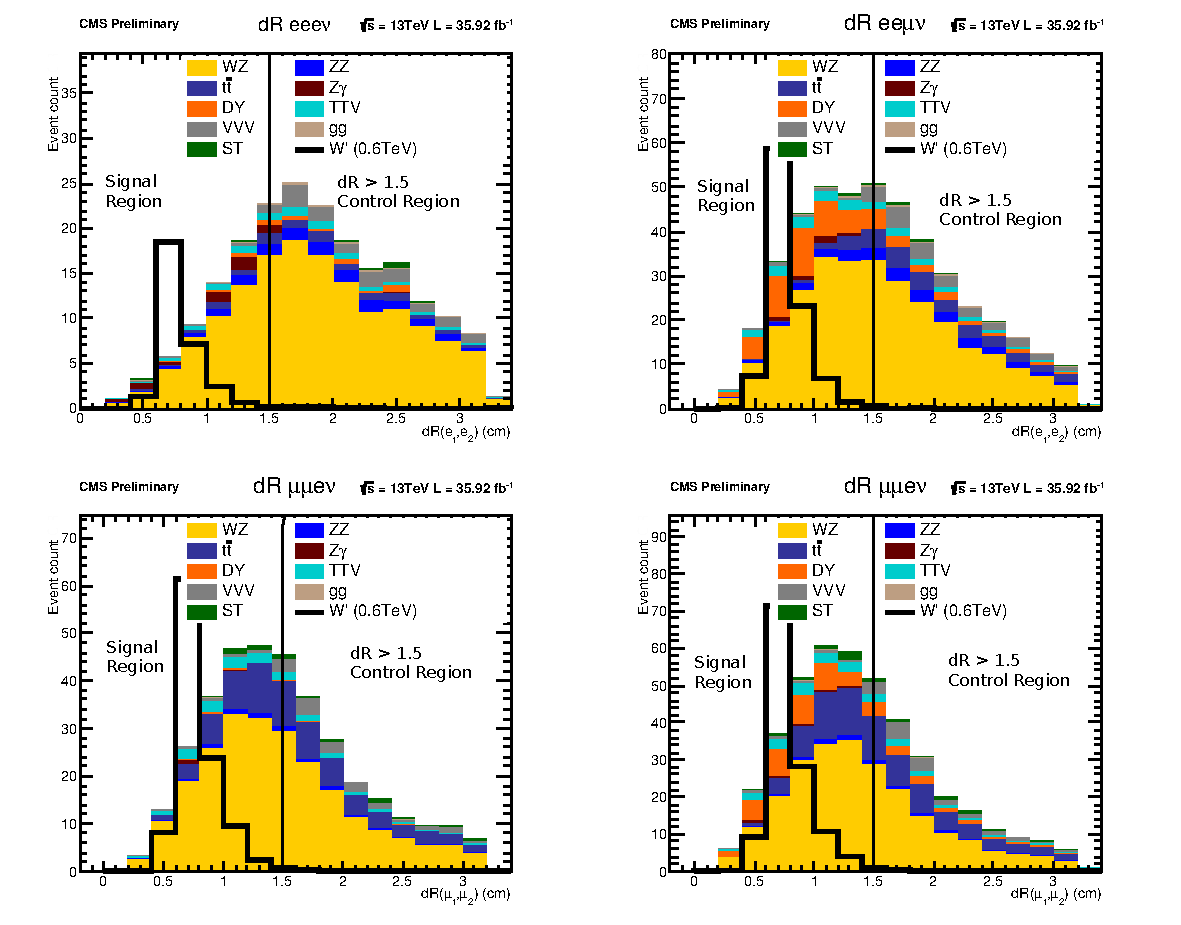
\includegraphics[width=\textwidth]{fig/Run2/KFactorIncluded_HDistl1l2_CR1_A+HDisM600.pdf}
  \caption{Definition of the signal and control regions. All the channels
    show how the region $dr_{l_{1}l_{2}} > 1.5$ is signal-depleted. A $600 GeV$
    mass resonance is used for illustration purposes. The larger the resonance
    mass, the narrower the signal distribution gets and it is shifted towards
    the lower $dR$ region as the leptons product of the $Z$ decay get closer
    forming a boosted topology.
    Top left: $Z(\rightarrow e+e)W(\rightarrow e+\nu)$
    Top right: $Z(\rightarrow e+e)W(\rightarrow \mu+\nu)$
    Bottom left: $Z(\rightarrow \mu+\mu)W(\rightarrow e+\nu)$
    Bottom right: $Z(\rightarrow \mu+\mu)W(\rightarrow \mu+\nu)$}
  \label{fig:ControlRegionDefinition}
\end{figure}

In order to analyse the simulation quality, the data/MC ratio is studied on
a signal-depleted control region. As Figure \ref{fig:ControlRegionDefinition}
shows, the distance in the $\eta-\phi$ plane between the products
of the Z boson decay $Z(\rightarrow l_{1}+l_{2})$ allow a distinct separation between a signal-enriched
region ($dr_{l_{1}l_{2}} <= 1.5$) and a signal depleted region
($dr_{l_{1}l_{2}} > 1.5$). The signal-delepted region is dominated mainly by
the SM WZ production process. Background yields for the control and signal are
shown on Table \ref{tab:BackgroundYieldsCR} and \ref{tab:BackgroundYieldsSR}

\begin{figure}[tph]
  \centering
  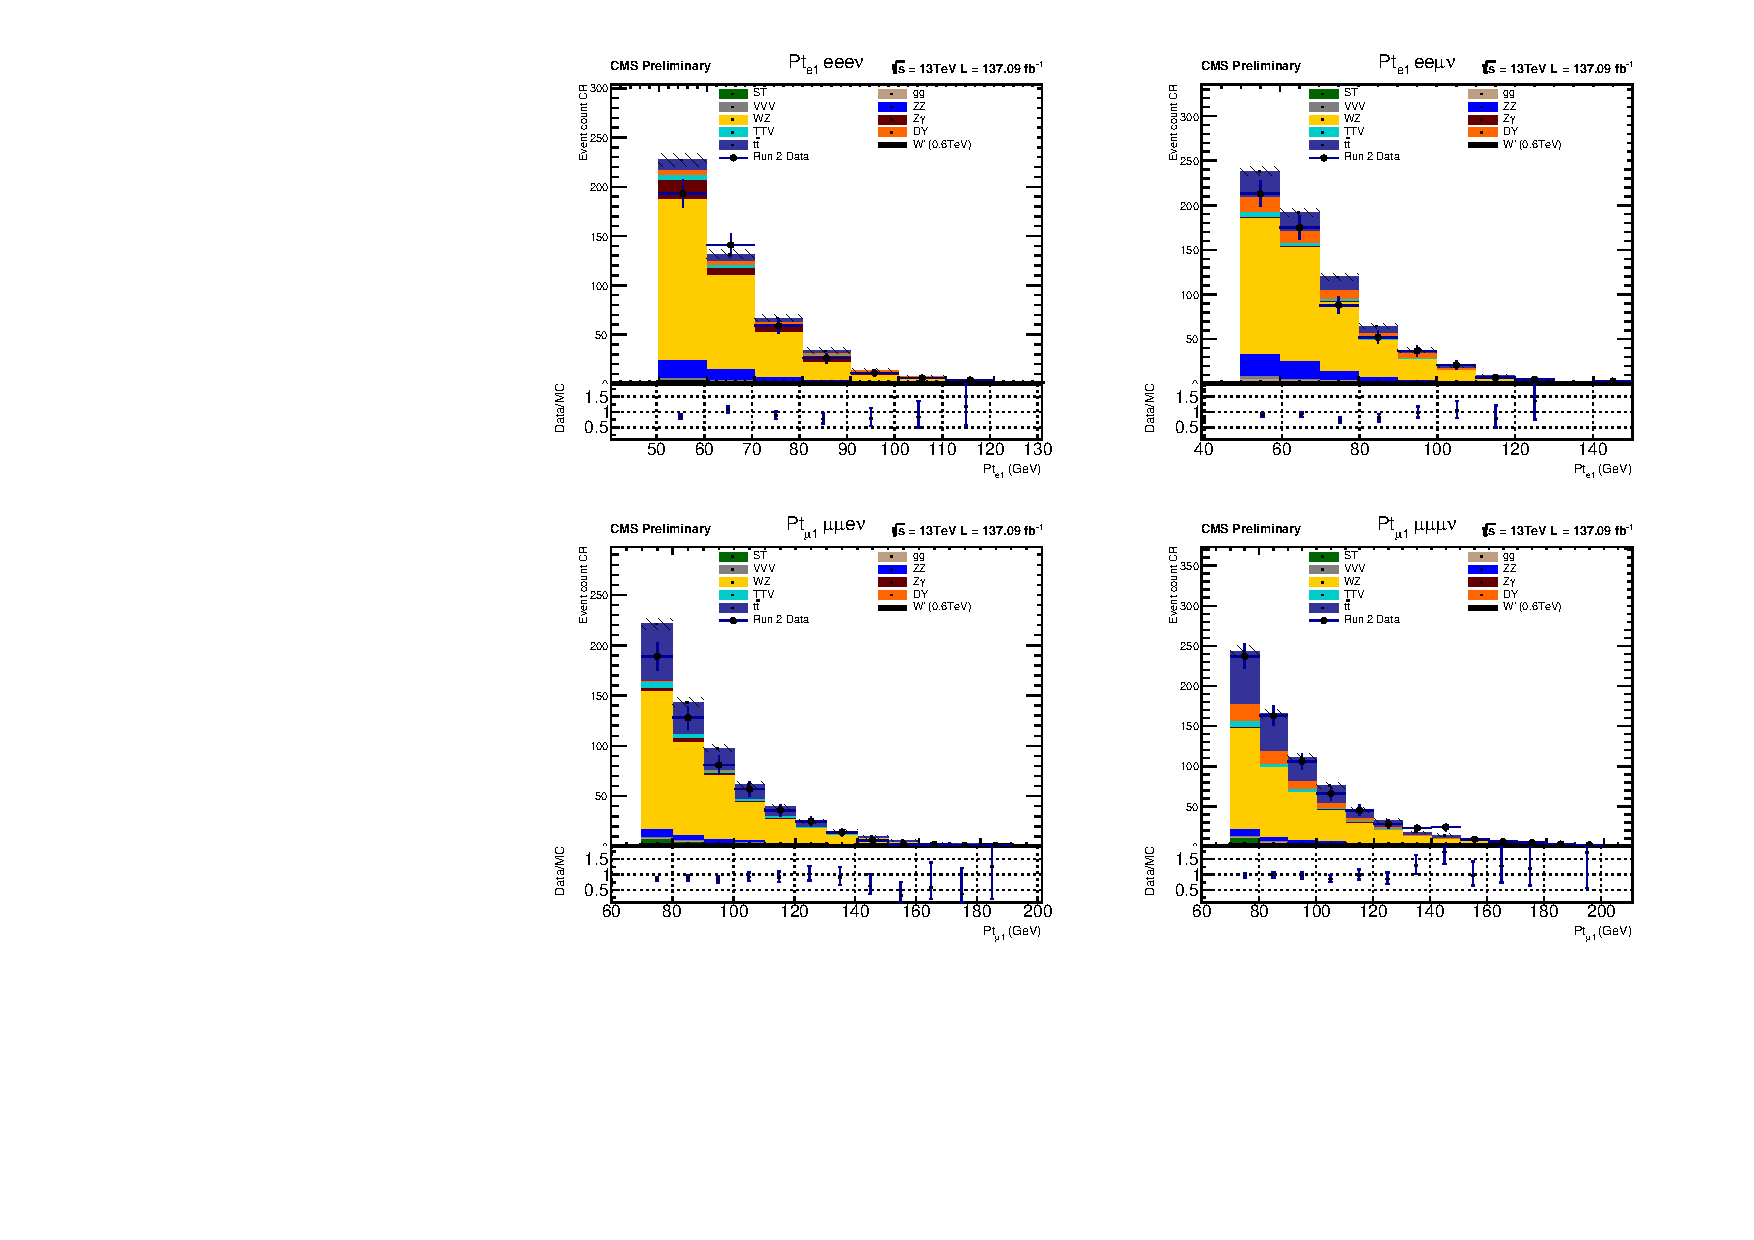
\includegraphics[width=\textwidth]{fig/Run2/KFactorIncluded_HPtl1_CR1_A_Run2_HPtRun2_M600.pdf}
  \caption{Leading lepton transverse momentum distributions for each final
    signature as seen in the $dr_{l_{1}l_{2}} > 1.5$ control region.
    Top left: $Z(\rightarrow e+e)W(\rightarrow e+\nu)$
    Top right: $Z(\rightarrow e+e)W(\rightarrow \mu+\nu)$
    Bottom left: $Z(\rightarrow \mu+\mu)W(\rightarrow e+\nu)$
    Bottom right: $Z(\rightarrow \mu+\mu)W(\rightarrow \mu+\nu)$}
  \label{fig:CR1_Run2_HPtl1}
\end{figure}

\begin{figure}[tph]
  \centering
  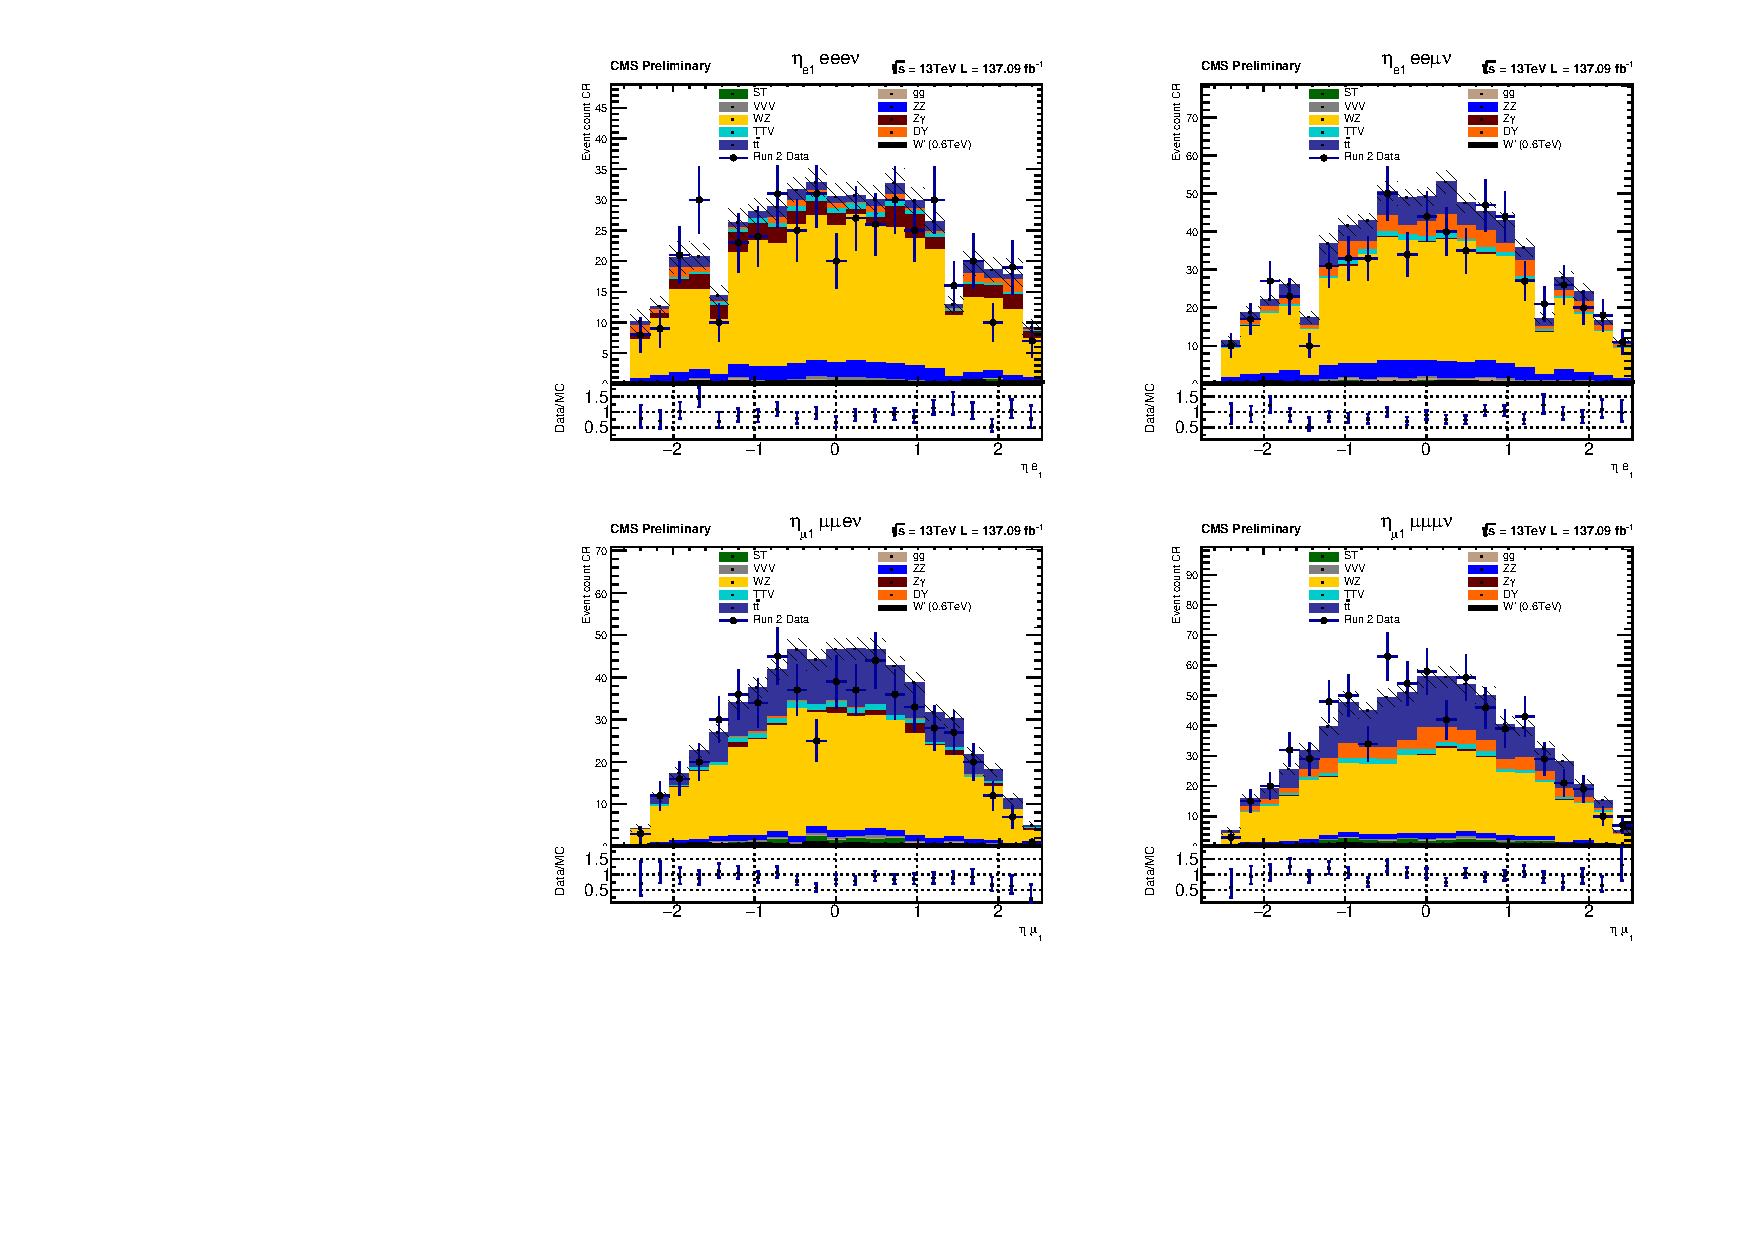
\includegraphics[width=\textwidth]{fig/Run2/KFactorIncluded_HEtal1_CR1_A_Run2_HERun2_M600.pdf}
  \caption{Leading lepton $\eta$ distributions for each final
    signature as seen in the $dr_{l_{1}l_{2}} > 1.5$ control region.
    Top left: $Z(\rightarrow e+e)W(\rightarrow e+\nu)$
    Top right: $Z(\rightarrow e+e)W(\rightarrow \mu+\nu)$
    Bottom left: $Z(\rightarrow \mu+\mu)W(\rightarrow e+\nu)$
    Bottom right: $Z(\rightarrow \mu+\mu)W(\rightarrow \mu+\nu)$}
  \label{fig:CR1_Run2_HEtal1}
\end{figure}

\begin{figure}[tph]
  \centering
  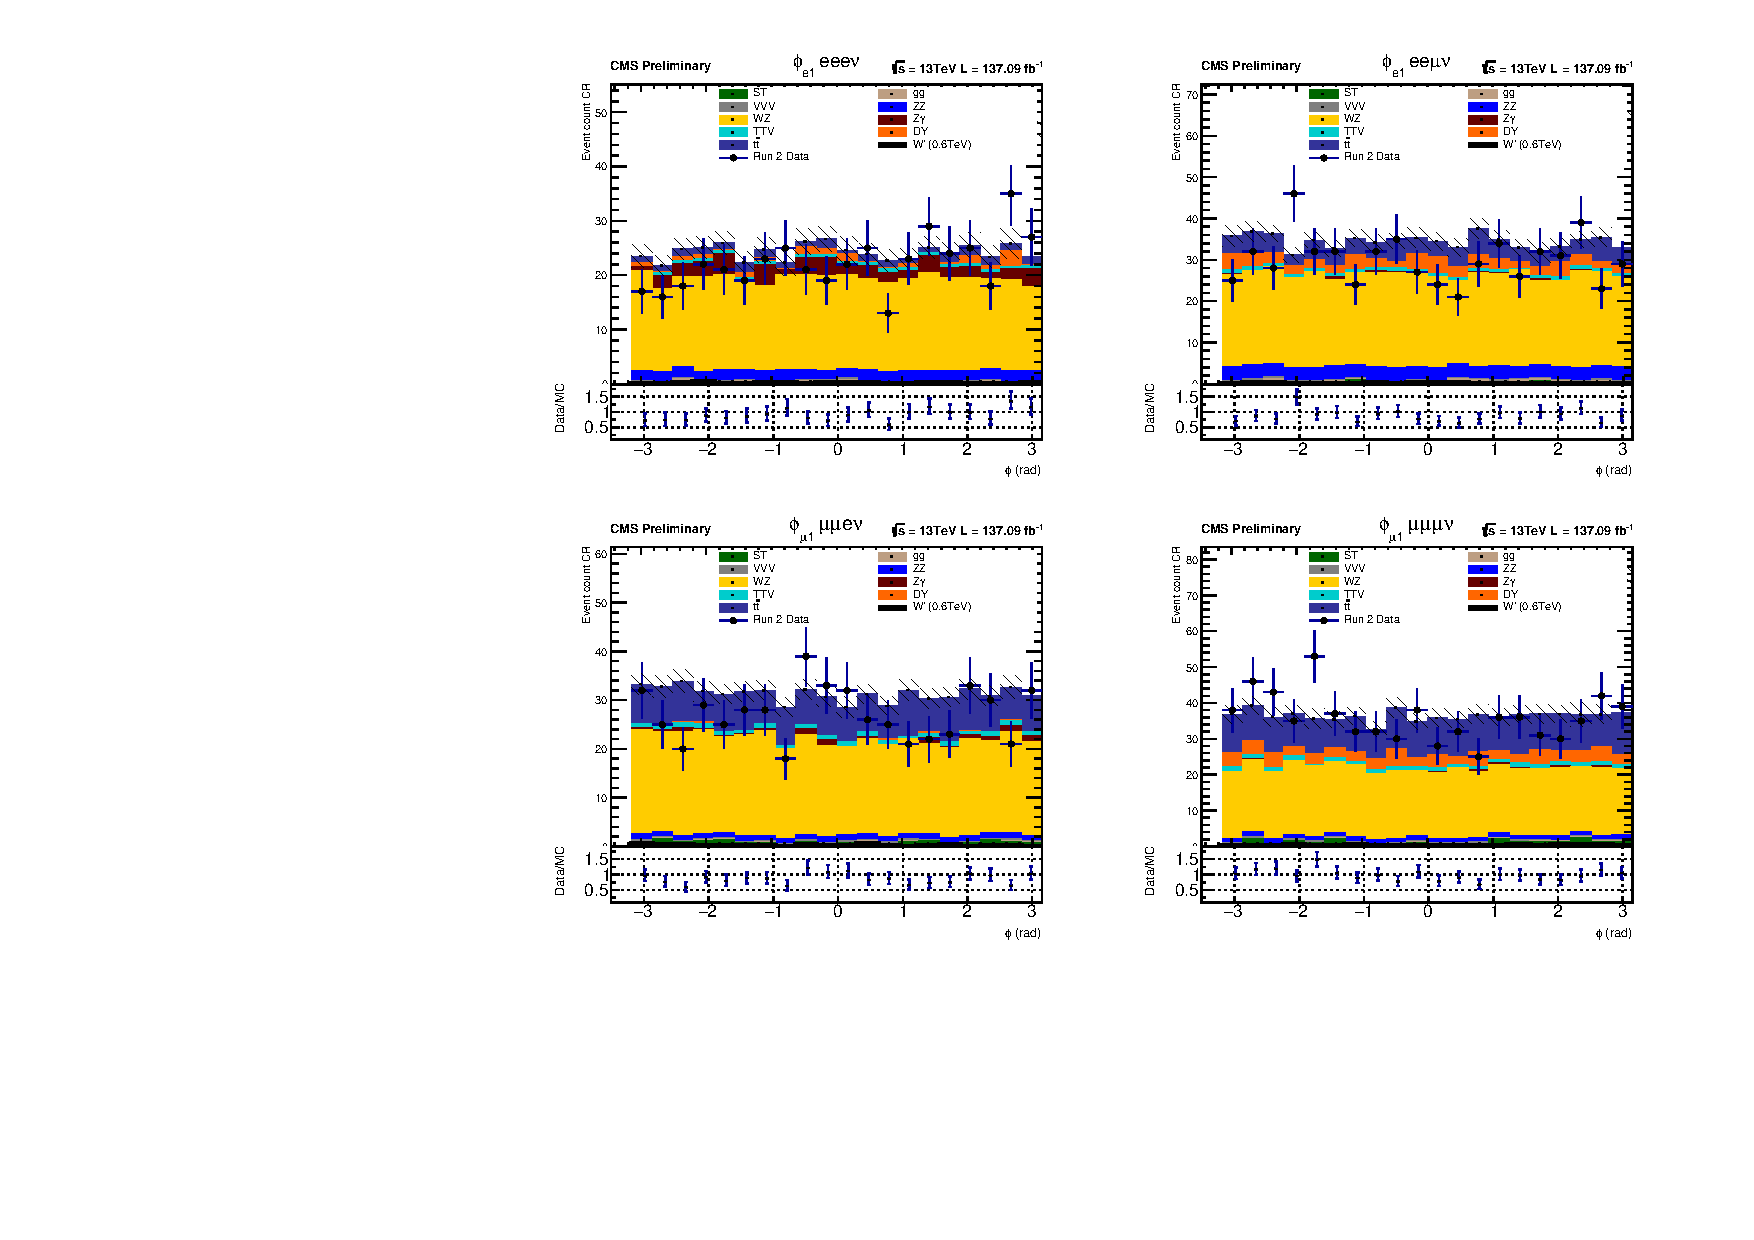
\includegraphics[width=\textwidth]{fig/Run2/KFactorIncluded_HPhil1_CR1_A_Run2_HPRun2_M600.pdf}
  \caption{Leading lepton $phi$ distributions for each final
    signature as seen in the $dr_{l_{1}l_{2}} > 1.5$ control region.
    Top left: $Z(\rightarrow e+e)W(\rightarrow e+\nu)$
    Top right: $Z(\rightarrow e+e)W(\rightarrow \mu+\nu)$
    Bottom left: $Z(\rightarrow \mu+\mu)W(\rightarrow e+\nu)$
    Bottom right: $Z(\rightarrow \mu+\mu)W(\rightarrow \mu+\nu)$}
  \label{fig:CR1_Run2_HPhil1}
\end{figure}

\begin{figure}[tph]
  \centering
  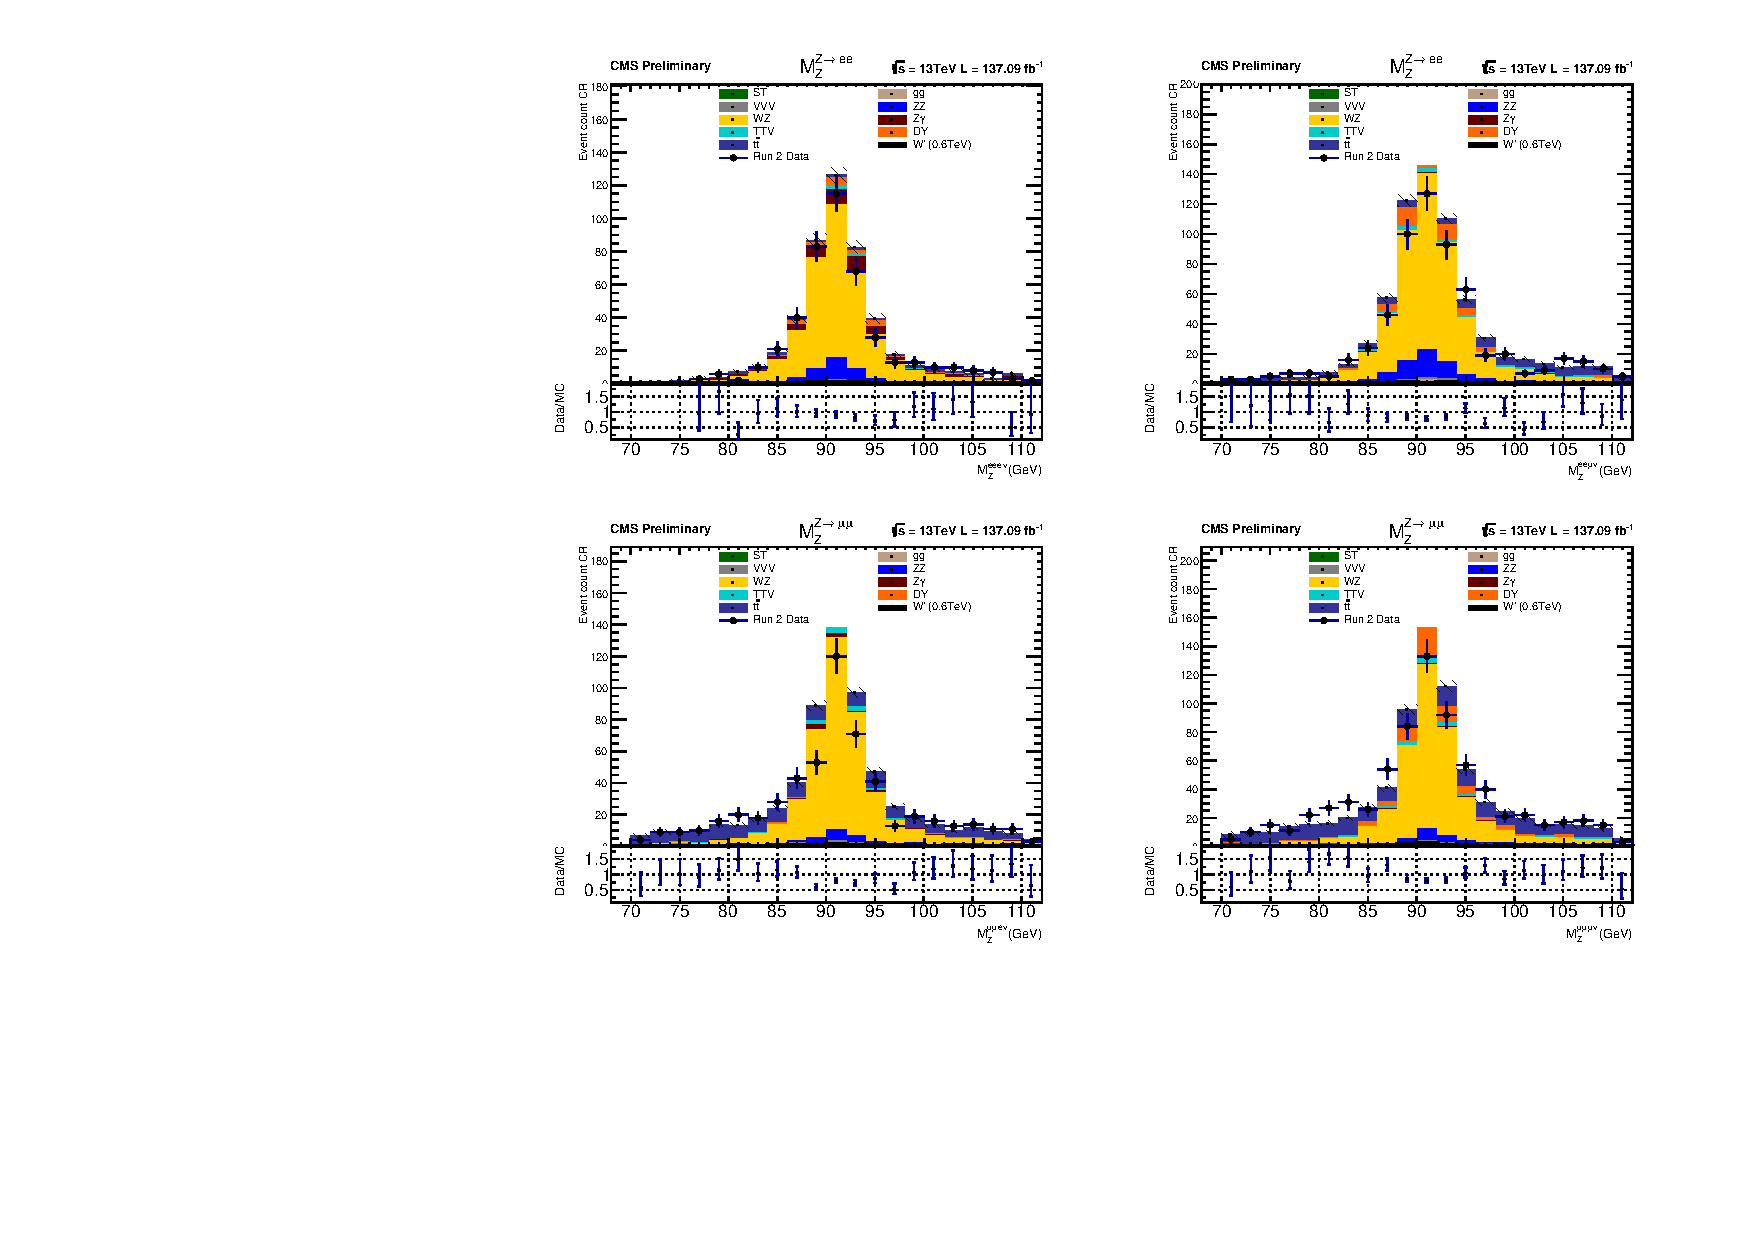
\includegraphics[width=\textwidth]{fig/Run2/KFactorIncluded_HMassZ_CR1_A_Run2_HMRun2_M600.pdf}
  \caption{$M_{Z}$ distributions of $Z\rightarrow\ell\ell$ candidates for each final
    signature as seen in the $dr_{l_{1}l_{2}} > 1.5$ control region.
    Top left: $Z(\rightarrow e+e)W(\rightarrow e+\nu)$
    Top right: $Z(\rightarrow e+e)W(\rightarrow \mu+\nu)$
    Bottom left: $Z(\rightarrow \mu+\mu)W(\rightarrow e+\nu)$
    Bottom right: $Z(\rightarrow \mu+\mu)W(\rightarrow \mu+\nu)$}
  \label{fig:CR1_Run2_HMassZ}
\end{figure}

\begin{figure}[tph]
  \centering
  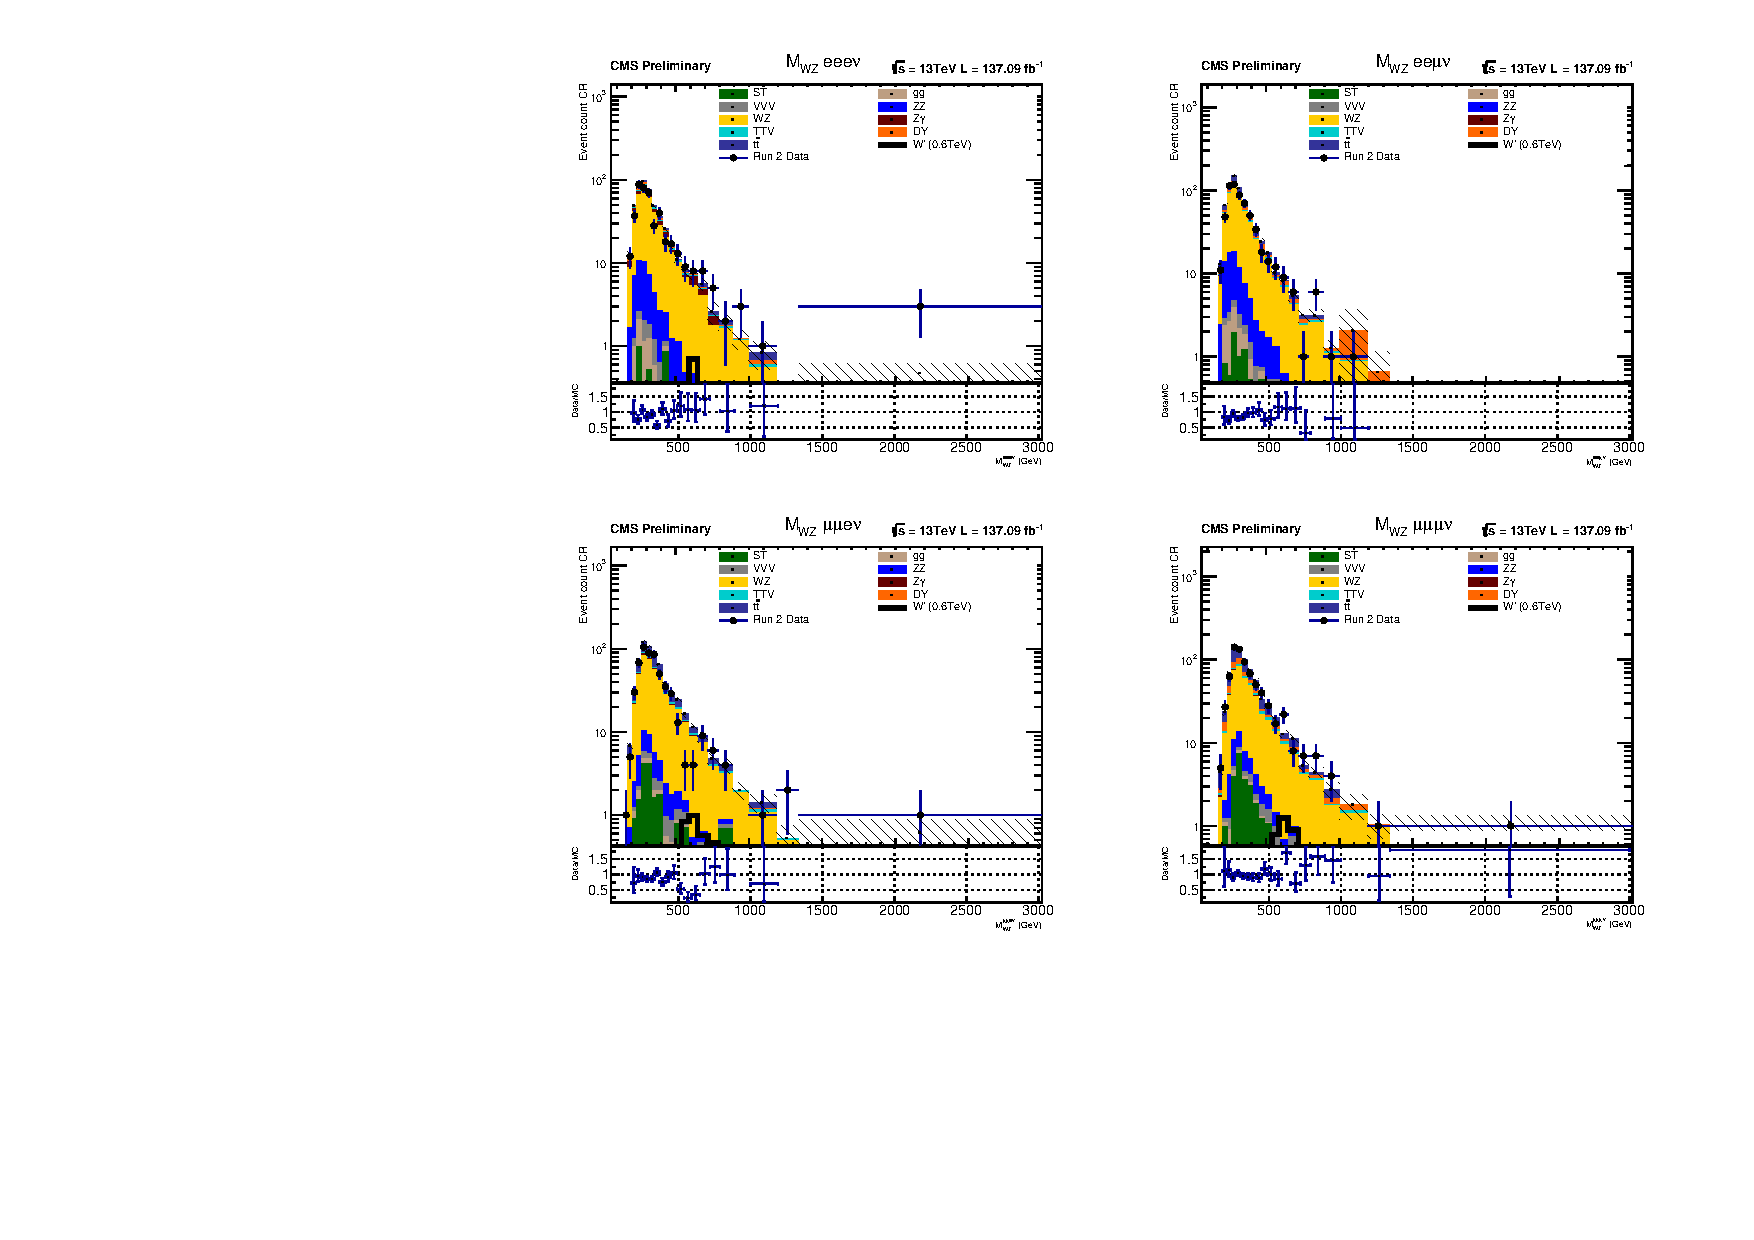
\includegraphics[width=\textwidth]{fig/Run2/Rebining_HMassWZ_CR1_A_Run2_HRun2_M600.pdf}
  \caption{The $WZ$ invariant mass after the $WZ$ candidate selection for each final
    signature as seen in the $dr_{l_{1}l_{2}} > 1.5$ control region.
    Top left: $Z(\rightarrow e+e)W(\rightarrow e+\nu)$
    Top right: $Z(\rightarrow e+e)W(\rightarrow \mu+\nu)$
    Bottom left: $Z(\rightarrow \mu+\mu)W(\rightarrow e+\nu)$
    Bottom right: $Z(\rightarrow \mu+\mu)W(\rightarrow \mu+\nu)$}
  \label{fig:CR1_Run2_HMassWZ}
\end{figure}

\begin{figure}[tph]
  \centering
  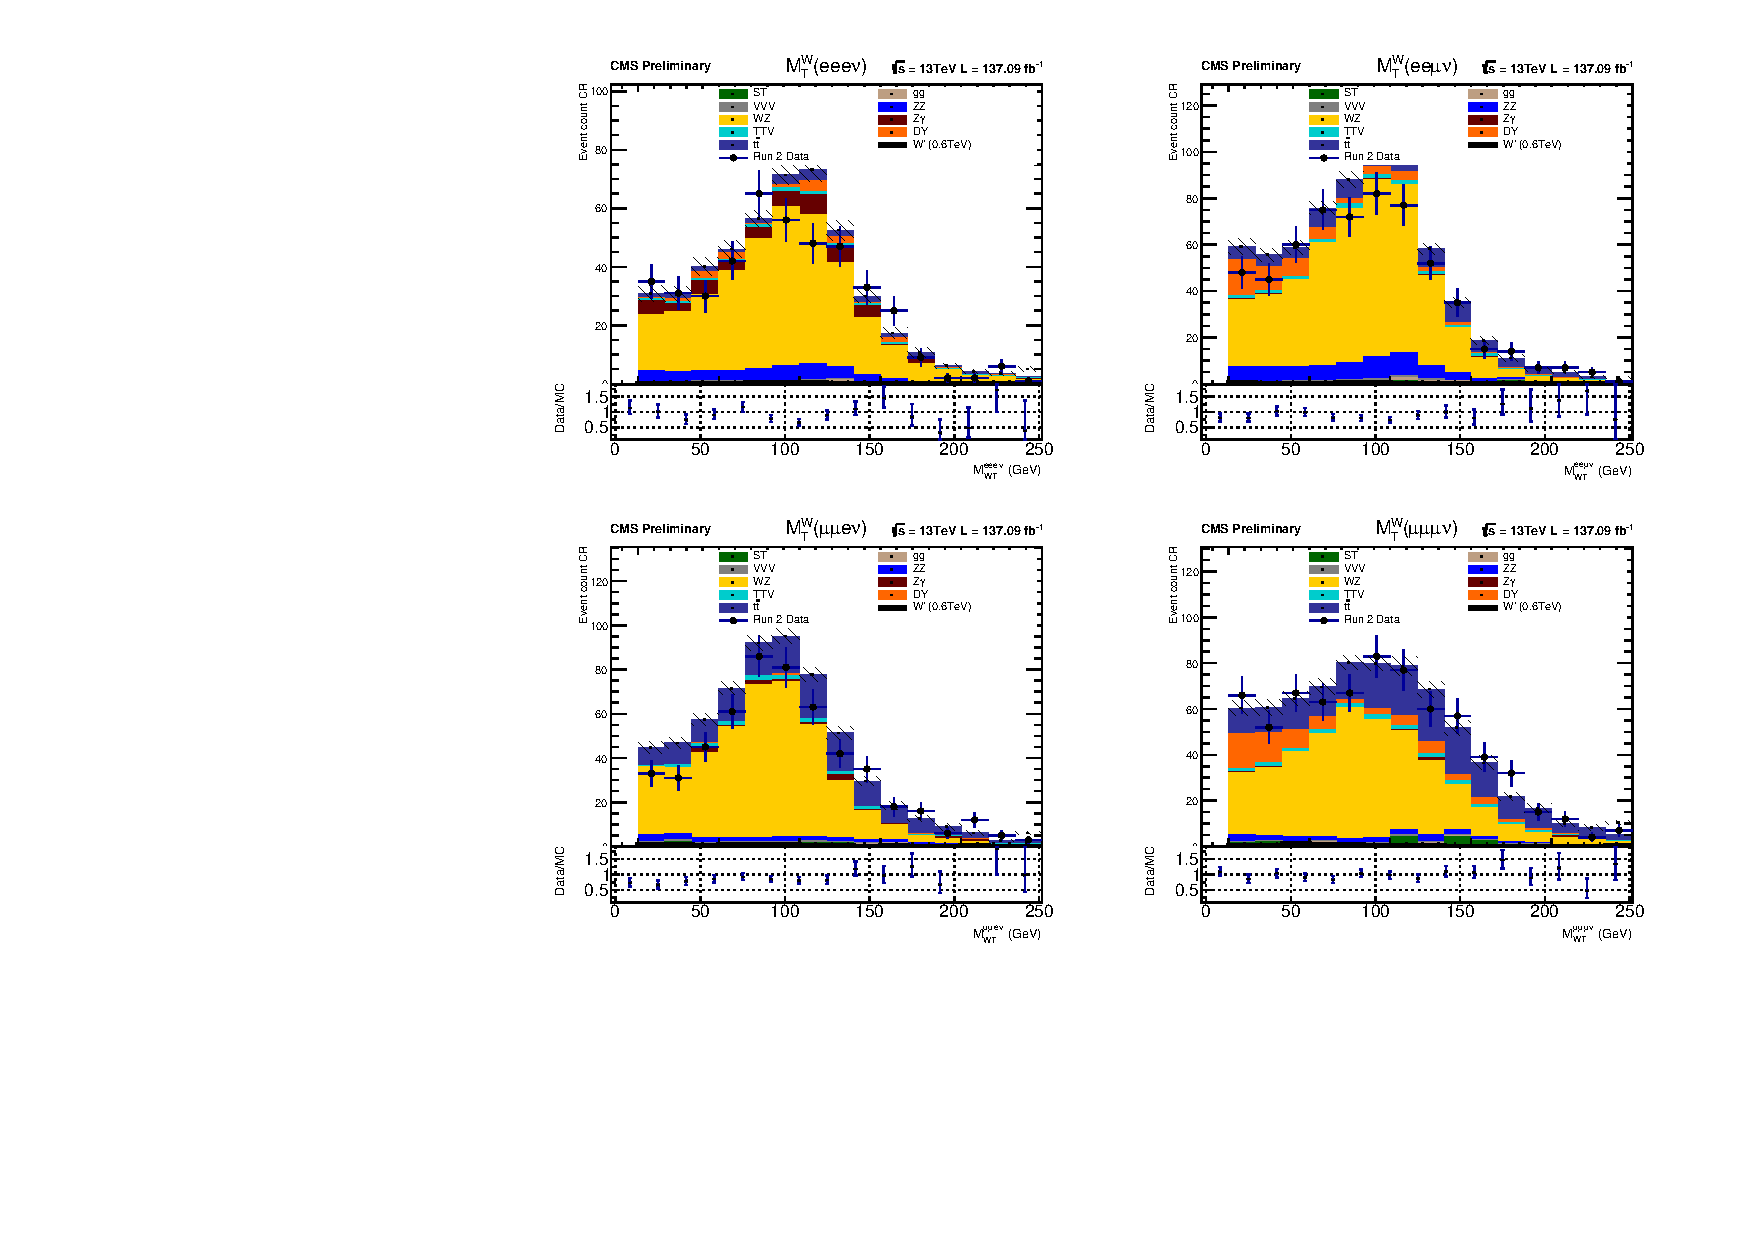
\includegraphics[width=\textwidth]{fig/Run2/KFactorIncluded_HMassTW_CR1_A_Run2_HRun2_M600.pdf}
  \caption{The transverse mass distribution for the $W$ candidate for each final
    signature as seen in the $dr_{l_{1}l_{2}} > 1.5$ control region.
    Top left: $Z(\rightarrow e+e)W(\rightarrow e+\nu)$
    Top right: $Z(\rightarrow e+e)W(\rightarrow \mu+\nu)$
    Bottom left: $Z(\rightarrow \mu+\mu)W(\rightarrow e+\nu)$
    Bottom right: $Z(\rightarrow \mu+\mu)W(\rightarrow \mu+\nu)$}
  \label{fig:CR1_Run2_HMassTW}
\end{figure}

The $\eta$, $\phi$, $P_{T}$ distributions for the leading lepton en each category
are shown in figures \ref{fig:CR1_Run2_HEtal1}, \ref{fig:CR1_Run2_HPhil1}, and
\ref{fig:CR1_Run2_HPtl1}, as well as composite distributions like the mass of the
reconstructed Z candidate (Figure \ref{fig:CR1_Run2_HMassZ}), the $W$ boson transverse mass
(Figure \ref{fig:CR1_Run2_HMassTW}) and the discriminant variable: the mass for the
reconstructed diboson system (Figure \ref{fig:CR1_Run2_HMassWZ}) show a good data/MC
agreement in the control region.


\begin{table}
  \caption{Background Yields per
    channel on Control Region}
 \begin{center}
 \begin{tabular}{cccccc}\hline\hline
Sample & $eee\nu$ & $ee\mu\nu$ & $\mu\mu e\nu$ & $\mu\mu\mu\nu$ & Total \\
DY & 15.87 & 53.38 & 2.09 & 65.86 & 137.19 \\
ST & 3.14 & 7.46 & 17.89 & 25.60 & 54.09 \\
TTV & 11.23 & 16.91 & 18.10 & 22.27 & 68.51 \\
VVV & 4.29 & 5.67 & 5.66 & 5.85 & 21.46 \\
WZ & 337.97 & 443.60 & 395.82 & 380.23 & 1,557.63 \\
$Z\gamma$ & 43.00 & 1.94 & 9.89 & 2.09 & 56.91 \\
ZZ & 38.58 & 65.07 & 22.31 & 25.54 & 151.50 \\
gg & 4.84 & 8.53 & 2.74 & 2.59 & 18.70 \\ \hline
Total Background & 458.91 & 602.57 & 474.50 & 530.03 & 2,066.01 \\ \hline
Total Data & 442.00 & 601.00 & 542.00 & 718.00 & 2,303.00 \\ \hline
 \end{tabular}
 \end{center}
 \label{tab:BackgroundYieldsCR}
\end{table}

\begin{table}
  \caption{Background Yields per
    channel on Signal Region}
 \begin{center}
 \begin{tabular}{cccccc}\hline\hline
Sample & $eee\nu$ & $ee\mu\nu$ & $\mu\mu e\nu$ & $\mu\mu\mu\nu$ & Total \\
DY & 9.88 & 225.94 & 225.94 & 232.50 & 694.26 \\
ST & 0.84 & 6.23 & 6.23 & 19.66 & 32.96 \\
TTV & 10.64 & 47.18 & 47.18 & 59.60 & 164.60 \\
VVV & 4.30 & 12.34 & 12.34 & 16.29 & 45.27 \\
WZ & 183.82 & 571.75 & 571.75 & 643.67 & 1,970.99 \\
$Z\gamma$ & 17.71 & 10.01 & 10.01 & 7.41 & 45.13 \\
ZZ & 18.74 & 47.29 & 47.29 & 30.69 & 144.01 \\
gg & 2.12 & 6.36 & 6.36 & 2.16 & 16.99 \\ \hline
Total Background & 248.04 & 927.11 & 927.11 & 1,011.96 & 3,114.22 \\ \hline
 \end{tabular}
 \end{center}
 \label{tab:BackgroundYieldsSR}
\end{table}
